\documentclass{article}

\usepackage{booktabs}
\usepackage{tabularx}
\usepackage{hyperref}
\usepackage{graphicx}
\usepackage{multirow}
\usepackage{pdflscape}
\usepackage[normalem]{ulem}
\graphicspath{./diagrams/}

\hypersetup{
    colorlinks=true,       % false: boxed links; true: colored links
    linkcolor=red,          % color of internal links (change box color with linkbordercolor)
    citecolor=green,        % color of links to bibliography
    filecolor=magenta,      % color of file links
    urlcolor=cyan           % color of external links
}

\title{Hazard Analysis\\\progname}

\author{\authname}

\date{}

%% Comments

\usepackage{color}

\newif\ifcomments\commentstrue %displays comments
%\newif\ifcomments\commentsfalse %so that comments do not display

\ifcomments
\newcommand{\authornote}[3]{\textcolor{#1}{[#3 ---#2]}}
\newcommand{\todo}[1]{\textcolor{red}{[TODO: #1]}}
\else
\newcommand{\authornote}[3]{}
\newcommand{\todo}[1]{}
\fi

\newcommand{\wss}[1]{\authornote{blue}{SS}{#1}} 
\newcommand{\plt}[1]{\authornote{magenta}{TPLT}{#1}} %For explanation of the template
\newcommand{\an}[1]{\authornote{cyan}{Author}{#1}}

%% Common Parts

\newcommand{\progname}{Software Engineering} % PUT YOUR PROGRAM NAME HERE
\newcommand{\authname}{Team 8 -- Rhythm Rangers\\
\\ Ansel Chen
\\ Muhammad Jawad
\\ Mohamad-Hassan Bahsoun
\\ Matthew Baleanu
\\ Ahmed Al-Hayali} % AUTHOR NAMES                  

\usepackage{hyperref}
    \hypersetup{colorlinks=true, linkcolor=blue, citecolor=blue, filecolor=blue,
                urlcolor=blue, unicode=false}
    \urlstyle{same}
                                


\begin{document}

\maketitle
\thispagestyle{empty}

~\newpage

\pagenumbering{roman}

\begin{table}[hp]
\caption{Revision History} \label{TblRevisionHistory}
\begin{tabularx}{\textwidth}{llX}
\toprule
\toprule {\textbf{Date}} & {\textbf{Version}} & {\textbf{Notes}}\\
\midrule
2024-10-25 & 0.0 & Revision 0\\
2025-04-04 & 1.0 & Revision 1, Fixed issues outlined under peer reviews \href{https://github.com/AhmedAl-Hayali/GenreGuru/issues/111}{Issue \#111}, \href{https://github.com/AhmedAl-Hayali/GenreGuru/issues/112}{Issue \#112}, \href{https://github.com/AhmedAl-Hayali/GenreGuru/issues/113}{Issue \#113}, \href{https://github.com/AhmedAl-Hayali/GenreGuru/issues/114}{Issue \#114}, \href{https://github.com/AhmedAl-Hayali/GenreGuru/issues/115}{Issue \#115}\\
\bottomrule
\end{tabularx}
\end{table}

~\newpage

\tableofcontents

~\newpage

\pagenumbering{arabic}

\section{Introduction}

This document is dedicated as a hazard analysis of the GenreGuru music system. The GenreGuru software is designed to aid its users with their consumption and creation of music, doing so by providing song analysis, recommendation, and music generation services. As such, we define a hazard as a potential malfunction in the system, either due to internal factors (such as the training data, defects in the software) or external factors (such as user inputs).

\section{Scope and Purpose of Hazard Analysis}
The purpose of hazard analysis for this project is to determine points and causes of failure in the system. \textcolor{red}{\sout{This includes their effects and considering mitigation methods.}} \textcolor{red}{This includes analyzing the effects of potential failures and devising appropriate mitigation strategies.} Here are some brief types of loss we expect hazards could incur: \\
\begin{itemize}
    \item Compromised Data -- such as corruption of the training dataset/outputs.
    \item Project History -- improper GitHub merging causing portions of documentation to vanish.
    \item User Experience Loss -- generated recommendations/snippets do not satisfy user needs.
\end{itemize}

\textcolor{red}{\sout{Note that traditional/physical hazards are not applicable in a pure software system.}} \textcolor{red}{It is important to note that traditional physical hazards (e.g., fires, explosions, mechanical failures) are not applicable in a pure software system such as this.}

\section{System Boundaries and Components}
\subsection{Diagrammatic System Characterization}
\begin{center}
    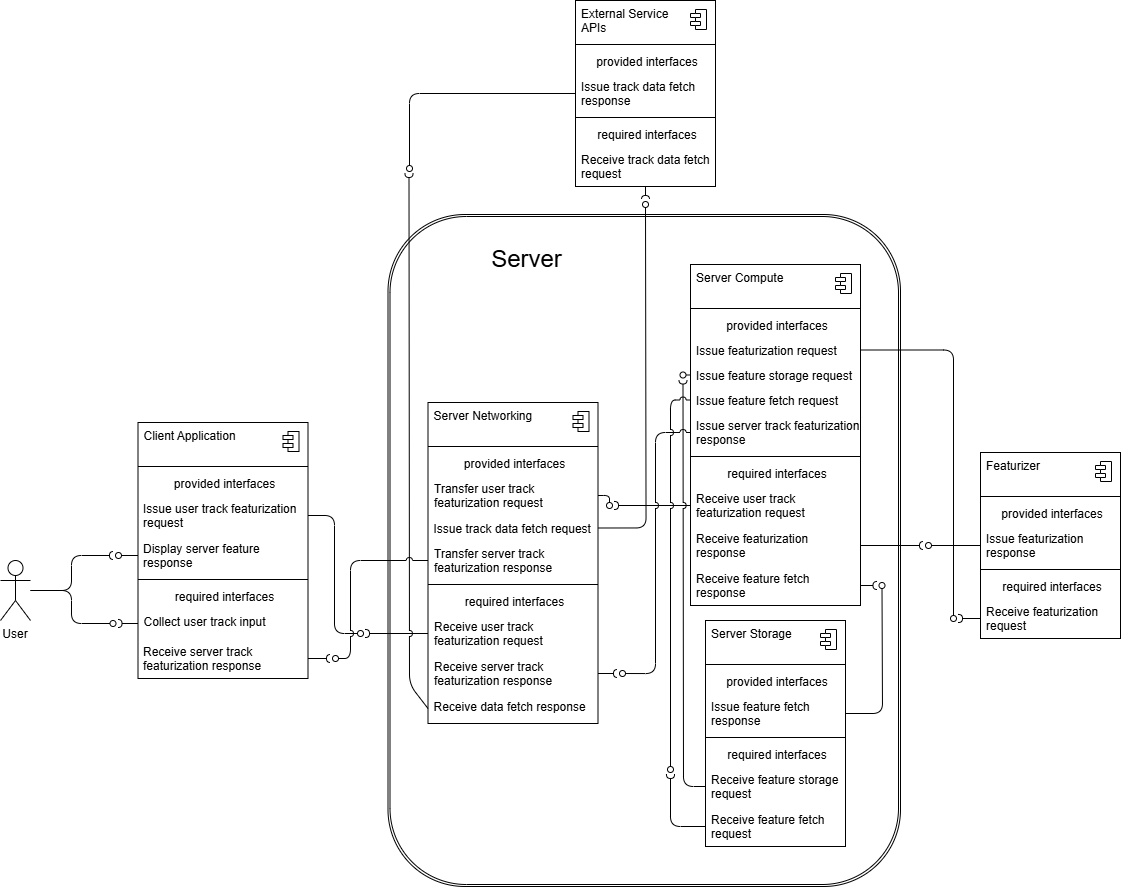
\includegraphics[width=\textwidth]{/diagrams/2_1_system_characterization_diagram.png}
\end{center}
\subsection{System Component Descriptions}
Please refer to table \ref{tbl:sys-cmpnt-desc}.
\begin{table}[h!]
    \centering
    \begin{tabular}{ p{.25\linewidth} || p{.65\linewidth} }
      \textbf{Component Name} & \textbf{Component Description} \\
      \toprule
      \emph{Client Application} & User-facing component through which they can input track information and view track features as system output. \\
      \midrule
      \emph{Server Networking} & Abstract component that represents communication between the server and external components, i.e., the client application and external service APIs. \\
      \midrule
      \emph{Server Compute} & Component that represents the server processing mechanism, i.e., the component that issues the featurization request. \\
      \midrule
      \emph{Server Storage} & Component that represents the server storage, i.e., the database. \\
      \midrule
      \emph{External Service APIs} & Component that represents external service APIs, e.g., the \href{https://developer.spotify.com/}{Spotify API} or \href{https://developers.deezer.com/}{Deezer API}. \\
      \midrule
      \emph{Featurizer} & Component that handles the featurization process.
    \end{tabular}
    \label{tbl:sys-cmpnt-desc}
    \caption{System Component Descriptions}
  \end{table}

\newpage
\section{Critical Assumptions}

\begin{itemize}
    \item \textcolor{red}{\sout{It is assumed that the user will not attempt to exploit system vulnerabilities to gain unauthorized access to the components of the system.}} \\
    \textcolor{red}{It is assumed that users will not intentionally misuse or attempt to break the system.}
    \item It is assumed that users will have the physical capabilities to interact with the system. \textcolor{red}{(Specifically, users are expected to have adequate visual acuity, fine motor control, and familiarity with input devices such as keyboards, mice, or touchscreens. Additionally, users must have access to hardware (e.g., a computer or smartphone) that meets the minimum display, processing, and connectivity requirements specified in the user documentation.)}
    \item It is assumed that all libraries used in development are \textcolor{red}{\sout{validated and tested.}} \textcolor{red}{validated and tested, where validation involves verifying that each library meets its documented functional and non-functional requirements (including API contracts and dependency compatibility), and testing involves comprehensive unit, integration, and regression tests to ensure stability and correct behavior under expected conditions.}
\end{itemize}

\section{Failure Mode and Effect Analysis}

\begin{landscape}
% Please add the following required packages to your document preamble:
% \usepackage{multirow}
\begin{table}[]
    \scalebox{.45}{
    \centering
    \begin{tabular}{|l|l|l|l|l|l|l|}
    \hline
    \multicolumn{1}{|c|}{Component} & \multicolumn{1}{c|}{Failure Mode} & \multicolumn{1}{c|}{Effects of Failure} & \multicolumn{1}{c|}{Causes of Failure} & \multicolumn{1}{c|}{Occurence (1-10)} & \multicolumn{1}{c|}{Severity (1-10)} & \multicolumn{1}{c|}{Detection (1-10)} \\ \hline
    \multirow{5}{*}{Client Application/User Interface} & \multirow{2}{*}{Unresponsive UI elements} & UI stops responding to user inputs & \multirow{2}{*}{Poor backend implementation} & \multirow{2}{*}{7} & \multirow{2}{*}{4} & \multirow{2}{*}{10} \\
     &  & User frustration &  &  &  &  \\ \cline{2-7} 
     & Incorrect display of data & Confuse users and lead to incorrect decisions & Data formatting or parsing errors from backend & 2 & 3 & 4 \\ \cline{2-7} 
     & \multirow{2}{*}{Transfer of User Request fails} & \multirow{2}{*}{Cannot Process User Request} & Invalid User Input & \multirow{2}{*}{1} & \multirow{2}{*}{10} & \multirow{2}{*}{4} \\
     &  &  & Server Failure &  &  &  \\ \hline
    \multirow{2}{*}{Featurizer} & Fail to extract any or all features of a particular input (similar to the one above) & Missing features degrades the quality/performance of the featurizer & Poor implementation, or bugs in the feature extraction process & 3 & 7 & 10 \\ \cline{2-7} 
     & Inconsistent feature outputs for the same input & Leads to unreliable song recommendations and system distrust & Improper configuration of random state & 3 & 7 & 10 \\ \hline
    \multirow{5}{*}{External Service APIs} & \multirow{5}{*}{API Request Failure} & \multirow{5}{*}{Service that requires API stops functioning} & \multirow{3}{*}{Hit Music Streaming Provider API rate limit} & \multirow{5}{*}{1} & \multirow{5}{*}{3} & \multirow{5}{*}{1} \\
     &  &  &  &  &  &  \\
     &  &  &  &  &  &  \\
     &  &  & \multirow{2}{*}{API Format/Version Changes} &  &  &  \\
     &  &  &  &  &  &  \\ \hline
    \multirow{3}{*}{Version Control System} & \multirow{2}{*}{Portions of Repository Are of Erroneous version} & \multirow{2}{*}{Section(s) of documentation are erroneously deleted} & \multirow{2}{*}{Improper merge conflict resolution within github} & \multirow{2}{*}{7} & \multirow{2}{*}{5} & \multirow{2}{*}{5} \\
     &  &  &  &  &  &  \\ \cline{2-7} 
     & Lack of commit message standards & Difficulties in tracking changes and debugging & No commit message policy or enforcement & 3 & 4 & 10 \\ \hline
    \multirow{3}{*}{Server Networking} & \multirow{3}{*}{Client Application cannot connect to server} & App gets stuck on current task & Server network module fails & \multirow{3}{*}{6} & \multirow{3}{*}{10} & \multirow{3}{*}{5} \\
     &  & \multirow{2}{*}{User Input is Lost} & Server loses power &  &  &  \\
     &  &  & Webapp device network module fails &  &  &  \\ \hline
    \multirow{4}{*}{Server Compute} & \multirow{3}{*}{Server timeout} & \multirow{3}{*}{No response from the server} & Server is overloaded & \multirow{3}{*}{4} & \multirow{3}{*}{10} & \multirow{3}{*}{6} \\
     &  &  & Server power loss &  &  &  \\
     &  &  & Poor computation logic &  &  &  \\ \cline{2-7} 
     & Network Latency/ High ping times & Slow response times and degraded user experience & Congested network or bandwidth limitations & 7 & 5 & 5 \\ \hline
    \multirow{7}{*}{Server Storage} & \multirow{2}{*}{Server storage is inaccessible} & \multirow{2}{*}{Server query failure} & Storage device failure & \multirow{2}{*}{1} & \multirow{2}{*}{10} & \multirow{2}{*}{10} \\
     &  &  & Server power loss &  &  &  \\ \cline{2-7} 
     & \multirow{2}{*}{Duplicate database entries} & \multirow{2}{*}{Compute unit returns incorrect information} & \multirow{2}{*}{Lack of duplicate protection} & \multirow{2}{*}{1} & \multirow{2}{*}{6} & \multirow{2}{*}{3} \\
     &  &  &  &  &  &  \\ \cline{2-7} 
     & \multirow{2}{*}{Data corruption} & Compute unit response contains errors or is empty & Server power loss & \multirow{2}{*}{1} & \multirow{2}{*}{10} & \multirow{2}{*}{7} \\
     &  & Data loss & Storage device failure &  &  &  \\ \cline{2-7} 
     & Data retrieval delay & Slow system response or timeouts during data access & Fragemented storage or high I/O usage & 10 & 3 & 8 \\ \hline
    \end{tabular}
    }
\end{table}

\begin{table}[hp]
    \centering
    \scalebox{.45}{
    \begin{tabular}{|l|l|l|l|l|l|}
    \hline
    \multicolumn{1}{|c|}{Component} & \multicolumn{1}{c|}{Failure Mode} & \multicolumn{1}{c|}{RPN} & \multicolumn{1}{c|}{Recommended Action(s)} & \multicolumn{1}{c|}{SR} & \multicolumn{1}{c|}{Ref.} \\ \hline
    \multirow{5}{*}{Client Application/User Interface} & \multirow{2}{*}{Unresponsive UI elements} & \multirow{2}{*}{280} & \multirow{2}{*}{Display a message to the user to refresh the page} & \multirow{2}{*}{} & \multirow{2}{*}{H1-1} \\
        &  &  &  &  &  \\ \cline{2-6} 
        & Incorrect display of data & 24 & Validate data before rendering and implement data consistency checks &  & H1-2 \\ \cline{2-6} 
        & \multirow{2}{*}{Transfer of User Request fails} & \multirow{2}{*}{40} & Implement Flexible Methods For User Inputs & \multirow{2}{*}{} & \multirow{2}{*}{H1-3} \\
        &  &  & Local Storage of User Requests for recovery &  &  \\ \hline
    \multirow{2}{*}{Featurizer} & Fail to extract any or all features of a particular input (similar to the one above) & 210 & Ensure featurizer algorithm is robust and well tested &  & H2-1 \\ \cline{2-6} 
        & Inconsistent feature outputs for the same input & 210 & Ensure featurizer algorithm is robust and thoroughly tested with diverse datasets &  & H2-2 \\ \hline
    \multirow{5}{*}{External Service APIs} & \multirow{5}{*}{API Request Failure} & \multirow{5}{*}{3} & Throttle API requests if there are a large amount of them & \multirow{5}{*}{} & \multirow{5}{*}{H3-1} \\
        &  &  & Minimize the amount of API calls the service makes &  &  \\
        &  &  & Fallbacks if API request denied (request post-poned instead of cancelled) &  &  \\
        &  &  & Monitor API Updates &  &  \\
        &  &  & Build flexbile code, rely on classes such that change occur in one location rather than all over the place &  &  \\ \hline
    \multirow{3}{*}{Version Control System} & \multirow{2}{*}{Portions of Repository Are of Erroneous version} & \multirow{2}{*}{175} & Use Github Branches & \multirow{2}{*}{} & \multirow{2}{*}{H4-1} \\
        &  &  & Proper Merge Conflict resolution &  &  \\ \cline{2-6} 
        & Lack of commit message standards & 120 & Enforce commit message templates &  & H4-2 \\ \hline
    \multirow{3}{*}{Server Networking} & \multirow{3}{*}{Client Application cannot connect to server} & \multirow{3}{*}{300} & Display message to user, attempt to reconnect to the server & \multirow{3}{*}{} & \multirow{3}{*}{H5-1} \\
        &  &  & \multirow{2}{*}{Regularly backup server storage} &  &  \\
        &  &  &  &  &  \\ \hline
    \multirow{4}{*}{Server Compute} & \multirow{3}{*}{Server timeout} & \multirow{3}{*}{240} & Display message to user to contact system administrator & \multirow{3}{*}{} & \multirow{3}{*}{H6-1} \\
        &  &  & Regularly backup server storage &  &  \\
        &  &  & Optimize processing algorithms &  &  \\ \cline{2-6} 
        & Network Latency/ High ping times & 175 & Implement Quality of Service (QoS) configurations and monitor bandwidth usage &  & H6-2 \\ \hline
    \multirow{7}{*}{Server Storage} & \multirow{2}{*}{Server storage is inaccessible} & \multirow{2}{*}{100} & Display message to user to contact system administrator & \multirow{2}{*}{IR1} & \multirow{2}{*}{H7-1} \\
        &  &  & Regularly backup server storage &  &  \\ \cline{2-6} 
        & \multirow{2}{*}{Duplicate database entries} & \multirow{2}{*}{18} & Implement duplicate protection measures & \multirow{2}{*}{IR2} & \multirow{2}{*}{H7-2} \\
        &  &  & Merge duplicate entries &  &  \\ \cline{2-6} 
        & \multirow{2}{*}{Data corruption} & \multirow{2}{*}{70} & \multirow{2}{*}{Regularly backup server storage} & \multirow{2}{*}{IR1} & \multirow{2}{*}{H7-3} \\
        &  &  &  &  &  \\ \cline{2-6} 
        & Data retrieval delay & 240 & Implement database indexing and optimize storage allocation &  & H7-4 \\ \hline
    \end{tabular}
    }
\end{table}
\end{landscape}

\section{Safety and Security Requirements}
Newly-added requirements are \emph{italicized}.
\subsection{Access Requirements}
\textbf{ACCR1.} The user shall only be able to access song features for songs they upload or ones that are licensed for their use.

\subsection{Integrity Requirements}
\emph{\textbf{IR1.} The server shall perform a weekly backup of its database to prevent data loss in the event of a catastrophic failure.} \\
\emph{\textbf{IR2.} The server shall implement deduplication measures to guarantee no data redundancy.}

\subsection{Privacy Requirements}
\textbf{PR1.} The system shall only expose query requests to the user that made them.

\subsection{Audit Requirements}
\textbf{AUR1.} The system shall maintain a history of user query requests.

\subsection{Immunity Requirements}
N/A.

\section{Roadmap}
As part of the capstone project timeline, we plan on implementing all safety requirements except for \emph{PR1} and \emph{AUR1}, which may be followed up on after May 2025.

\newpage{}

\section*{Appendix --- Reflection}

The purpose of reflection questions is to give you a chance to assess your own
learning and that of your group as a whole, and to find ways to improve in the
future. Reflection is an important part of the learning process.  Reflection is
also an essential component of a successful software development process.  

Reflections are most interesting and useful when they're honest, even if the
stories they tell are imperfect. You will be marked based on your depth of
thought and analysis, and not based on the content of the reflections
themselves. Thus, for full marks we encourage you to answer openly and honestly
and to avoid simply writing ``what you think the evaluator wants to hear.''

Please answer the following questions.  Some questions can be answered on the
team level, but where appropriate, each team member should write their own
response:


\begin{enumerate}
    \item What went well while writing this deliverable?
    
    The majority of the team was involved in collaborating to complete all sections of the deliverable together, as opposed to appointing different sections to different people. As a result, we engaged in a deep discussion regarding project scope and system components, prompting us to restrict our scope to just the featurization component, making the music recommendation and generation components stretch goals.

    \item What pain points did you experience during this deliverable, and how did you resolve them?
    
    Because the team was heavily engaged in collaborative completion of the document, there repeatedly were extended conversations during which we refined project scope, but also lost focus -- the loss of focus resulted in the deliverable taking a longer time to complete than would have otherwise been necessary.

    \item Which of your listed risks had your team thought of before this deliverable, and which did you think of while doing this deliverable? For the latter ones (ones you thought of while doing the Hazard Analysis), how did they come about?
    
    We fortunately were thorough in our consideration of hazards and risks while drafting prior deliverables. As a result, section 15 of our SRS document had considerable coverage except for two integrity requirements concerning data accuracy and persistence. When considering the server storage component of the system, we noted that there was no guarantee of data correctness or persistence should a server failure occur. As a result, we included IR1 and IR2 to capture these risks.

    \item Other than the risk of physical harm (some projects may not have any appreciable risks of this form), list at least 2 other types of risk in software products. Why are they important to consider?
    
    Two types of risks in software products that aren't related to physical are: the risk of compromising (user or software) data, and scope creep, where the software uncontrollably grows and developers commit to adding features beyond what was intially agreed to.
    \begin{enumerate}
        \item Data compromise is crucial to consider because user and application data can be very sensitive, e.g., users often reuse their credentials, thus said data being compromised could have far-reaching effects beyond just the user's ability to interact with the service. Company Data can also be very valuable, if it is exposed it could be used by competitors or used to exploit other vulnerabilities within the software. Compromising unreleased songs can also result in legal action being carried out against the devlopment team.
        \item Scope creep is important to consider because it arises when the project is not properly  defined during early planning stages. This often leads to extra developement work and accrual of costs for features that might not work properly or are unecessary for project success.
    \end{enumerate}
\end{enumerate}

\end{document}